\documentclass[9pt]{beamer}
\usepackage[utf8x]{inputenc}
\usepackage{xspace}
\usepackage{tikz}
\usepackage{relsize}
\usepackage{comment}
\usepackage[vlined,linesnumbered]{algorithm2e}
\usepackage{url}

\definecolor{red9}{rgb}{.9,0.2,0.2}
\definecolor{orange9}{HTML}{FF7522}
\definecolor{blue9}{HTML}{366690}
\definecolor{yellow9}{HTML}{E1B640}

\newcommand{\memph}[1]{{\color{yellow9}{\bf #1}}\xspace}

\usepackage{comment}

\mode<presentation>
{
  \setbeamercovered{transparent}
  \setbeamercolor{normal text}{fg=white,bg=gray}
  \setbeamercolor{alerted text}{fg=white}
  \setbeamercolor{example text}{fg=white,bg=blue9}
  \setbeamercolor{background canvas}{bg=darkgray} 
  \setbeamercolor{structure}{fg=white}

  \setbeamercolor{block title}{bg=blue9,fg=white}
  \setbeamercolor{block body}{bg=white,fg=darkgray}

  \setbeamercolor{palette primary}{use=structure,fg=structure.fg}

  \setbeamercolor{math text}{}
  \setbeamercolor{math text inlined}{parent=math text}
  \setbeamercolor{math text displayed}{parent=math text}

  \setbeamercolor{normal text in math text}{}

  \setbeamercolor{local structure}{parent=structure}

  \setbeamercolor{titlelike}{parent=structure}

  \setbeamercolor{title}{parent=titlelike}
  \setbeamercolor{title in head/foot}{parent=palette quaternary}
  \setbeamercolor{title in sidebar}{parent=palette sidebar quaternary}

  \setbeamercolor{subtitle}{parent=title}
}

\usefonttheme{serif}

%%%%%%%%%%%%%%%%%%%%%%%%%%%%%%
% Presentation Title Content %
%%%%%%%%%%%%%%%%%%%%%%%%%%%%%%
\title{Gröbner Bases}
\author[Martin R.\ Albrecht]{Martin R.\ Albrecht}
\institute[] % (optional, but mostly needed)
{DTU Crypto Group}

\date{22 October 2013}

\AtBeginSection[] {
	\begin{frame}
		\frametitle{Contents}
		\tableofcontents[sectionstyle=show/shaded,subsectionstyle=show/show/hide]
	\end{frame}
}

%% LISTINGS

\usepackage{listings}
\lstdefinelanguage{Sage}[]{Python}{morekeywords={True,False,sage,cdef,cpdef,ctypedef,self},sensitive=true}
\lstset{frame=none,
          showtabs=False,
          showspaces=False,
          showstringspaces=False,
          commentstyle={\color{yellow9}},
          keywordstyle={\color{lightgray}},
          stringstyle ={\color{lightgray}},
          language = Sage,
          basicstyle=\footnotesize\tt
          }

%% NOTATION

\newcommand{\Q}{\ensuremath{\mathbb{Q}}\xspace}
\newcommand{\F}[1][]{\ensuremath{\mathbb{F}_{#1}}\xspace}
\newcommand{\Z}{\ensuremath{\mathbb{Z}}\xspace}
\newcommand{\I}{\ensuremath{\mathcal{I}}\xspace}
\newcommand{\gens}{\ensuremath{x_1,\dots,x_{n}}\xspace}
\newcommand{\LM}[1]{\ensuremath{\textsc{LM}\left(#1\right)}\xspace}
\newcommand{\LC}[1]{\ensuremath{\textsc{LC}\left(#1\right)}\xspace}
\newcommand{\LT}[1]{\ensuremath{\textsc{LT}\left(#1\right)}\xspace}
\newcommand{\LCM}[1]{\ensuremath{\textsc{LCM}(#1)\xspace}}
\newcommand{\ideal}[1]{\ensuremath{\langle #1\rangle}\xspace}

\begin{document}

\begin{frame}[plain] % frame of type 'plain' is an empty frame
  \titlepage
\end{frame}

\section{Sage}

\begin{frame}
\frametitle{Why not \dots}

This course involves implementing algorithms in multivariate polynomial rings for which we will be using the Sage mathematics software.

\vspace{1em}

You already know Maple, so why not use it?

\begin{enumerate}
 \item I do not know Maple so I could not help you with problems you might encounter.
 \item Maple is an expensive piece of software that you might not have access to outside of this university, cutting you off the tool you know. Sage does not have this problem.
 \item Maple is a closed source piece of software which means you cannot study, learn from and improve it. This goes against fundamental principles of reproducible science.
\end{enumerate}

\end{frame}


\begin{frame}
\frametitle{Blurb}

\begin{columns}

\column{0.15\textwidth}

\begin{center}
 
\includegraphics[height=0.9\textwidth]{./sage-logo.png}
\vspace{0.5em}
\end{center}

\column{0.8\textwidth}
\begin{block}{Sage open-source mathematical software system}
``Creating a viable free open source alternative to Magma, Maple, Mathematica and Matlab.''
\end{block}
\end{columns}

\vspace{1em}

Sage is a free open-source mathematics software system licensed under the GPL. It combines the power of many existing open-source packages into a common Python-based interface.

\vspace{1em}

\begin{tabular}{ll}
First release 2005 & Latest version 5.11 released 2013-08-13\\
$>$ 300 releases  & Shell, webbrowser (GUI), library\\
$>$ 180 developers  & $\sim 100$ components\\
$>$ 200 papers cite Sage & $> 2100$ subscribers [sage-support]\\
$>$ 100,000 web visitors/month&  $> 6,500$ downloads/month\\
\end{tabular}
\end{frame}

\begin{frame}[fragile]
\frametitle{Python \& Cython}
\begin{block}{}
\centering
 
\includegraphics[width=0.4\textwidth]{python-and-cython.png}
\end{block}

Sage does \memph{not} come with yet-another ad-hoc mathematical programming language, it uses
\memph{Python} instead.

\begin{itemize}
\item one of the most widely used programming languages (Google, IML, YouTube, NASA),
\item easy for you to define your own data types and methods on it (bitstreams, ciphers, rings, whatever),
\item very clean language that results in easy to read code,
\item a \memph{huge number of libraries}: statistics, networking, databases,
bioinformatic, physics, video games, 3d graphics, numerical computation (scipy),
and serious ``pure'' mathematics (via Sage)
\item easy to use existing C/C++ libraries from Python (via \memph{Cython})
\end{itemize}
\end{frame}


\begin{frame}[allowframebreaks,fragile]
\frametitle{How to use Sage}

Use Sage via
\begin{itemize}
 \item as a \memph{command line} programme, 
 \item as a \memph{webapp} hosted on your local computer and 
 \item as a webapp \memph{on the Internet}
\end{itemize}

\framebreak

To install Sage on your computer head to 
\begin{center}
\url{http://sagemath.org} 
\end{center}

and download the right version for your operating system\\
(Mac OS X, Windows, Linux \dots)

\vspace{1em}

You can then either run Sage on the \memph{command line} or start a \memph{local webapp}.

\framebreak

Calling \lstinline[language=bash,basicstyle=\tt]|sage|

\begin{center}
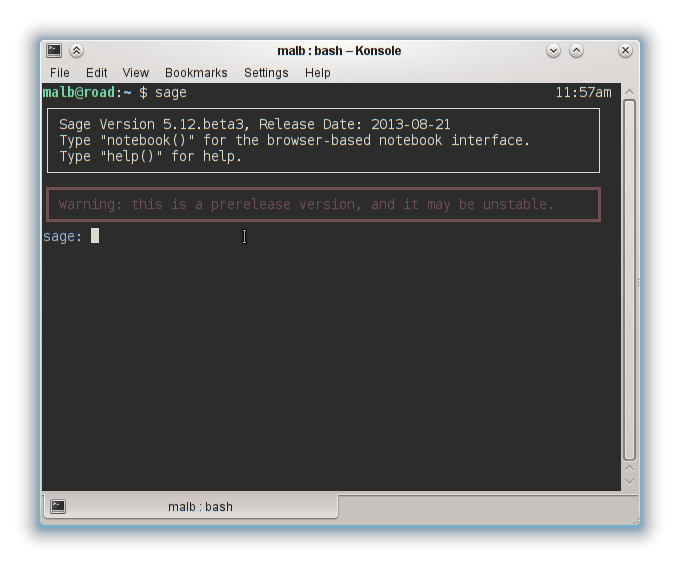
\includegraphics[width=0.6\textwidth]{sage-cli.png}
\end{center}

\framebreak

Calling \lstinline[language=bash,basicstyle=\tt]|sage -notebook|

\begin{center}
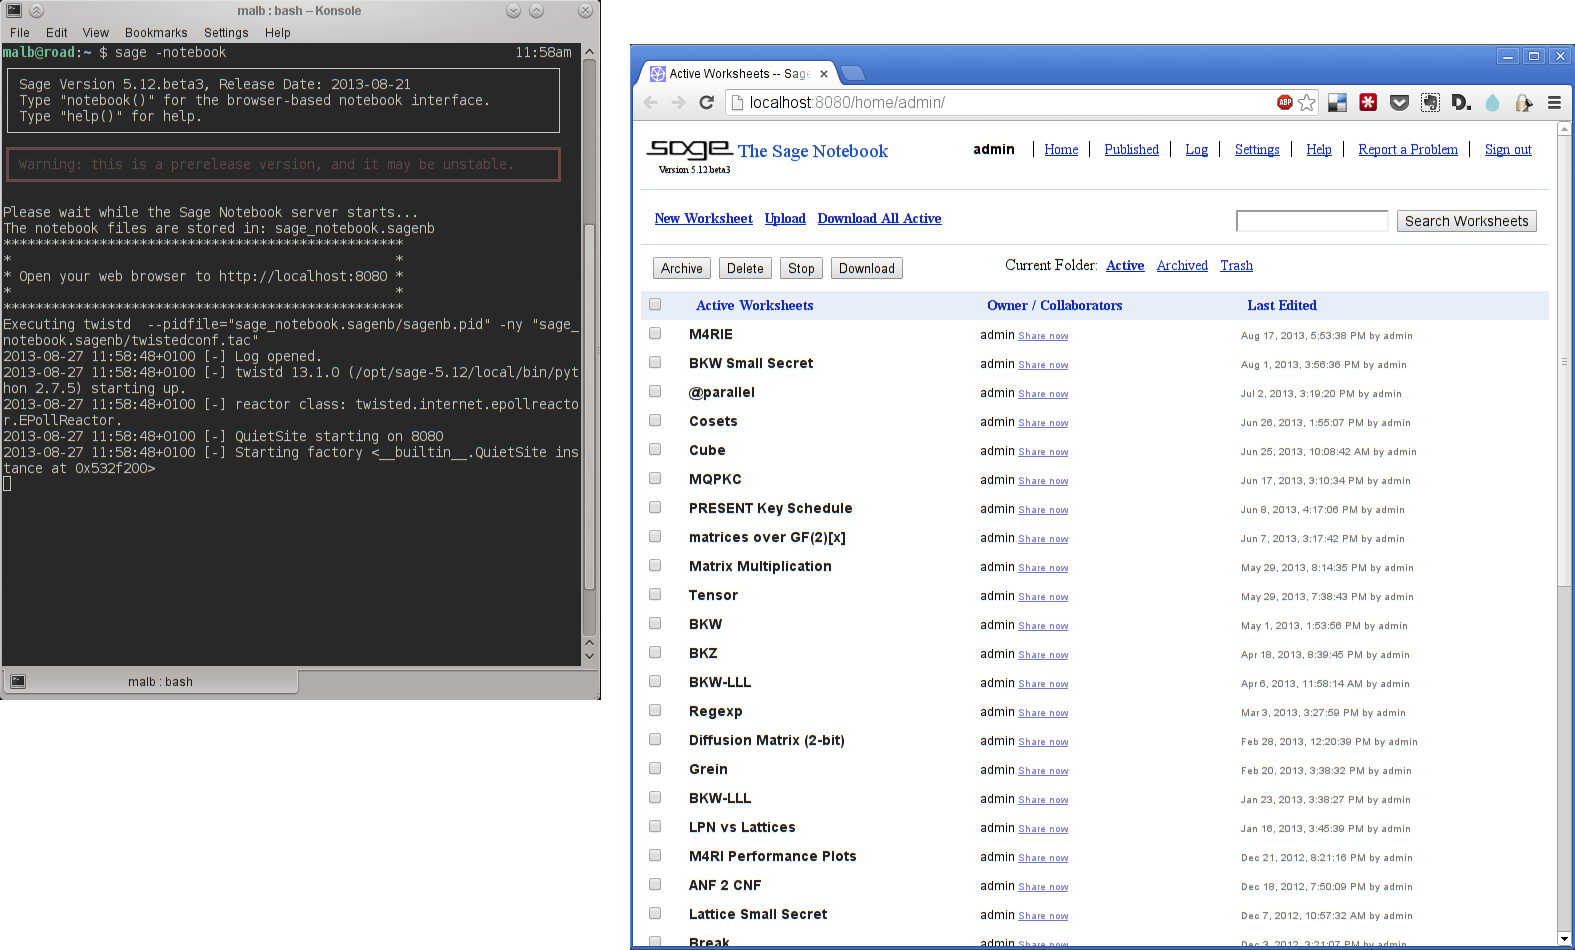
\includegraphics[width=\textwidth]{sage-webapp.png}
\end{center}

\framebreak

You can also use Sage online:
\begin{center}
\url{http://www.sagenb.org/}  and \url{https://cloud.sagemath.com/}
\end{center}

\begin{center}
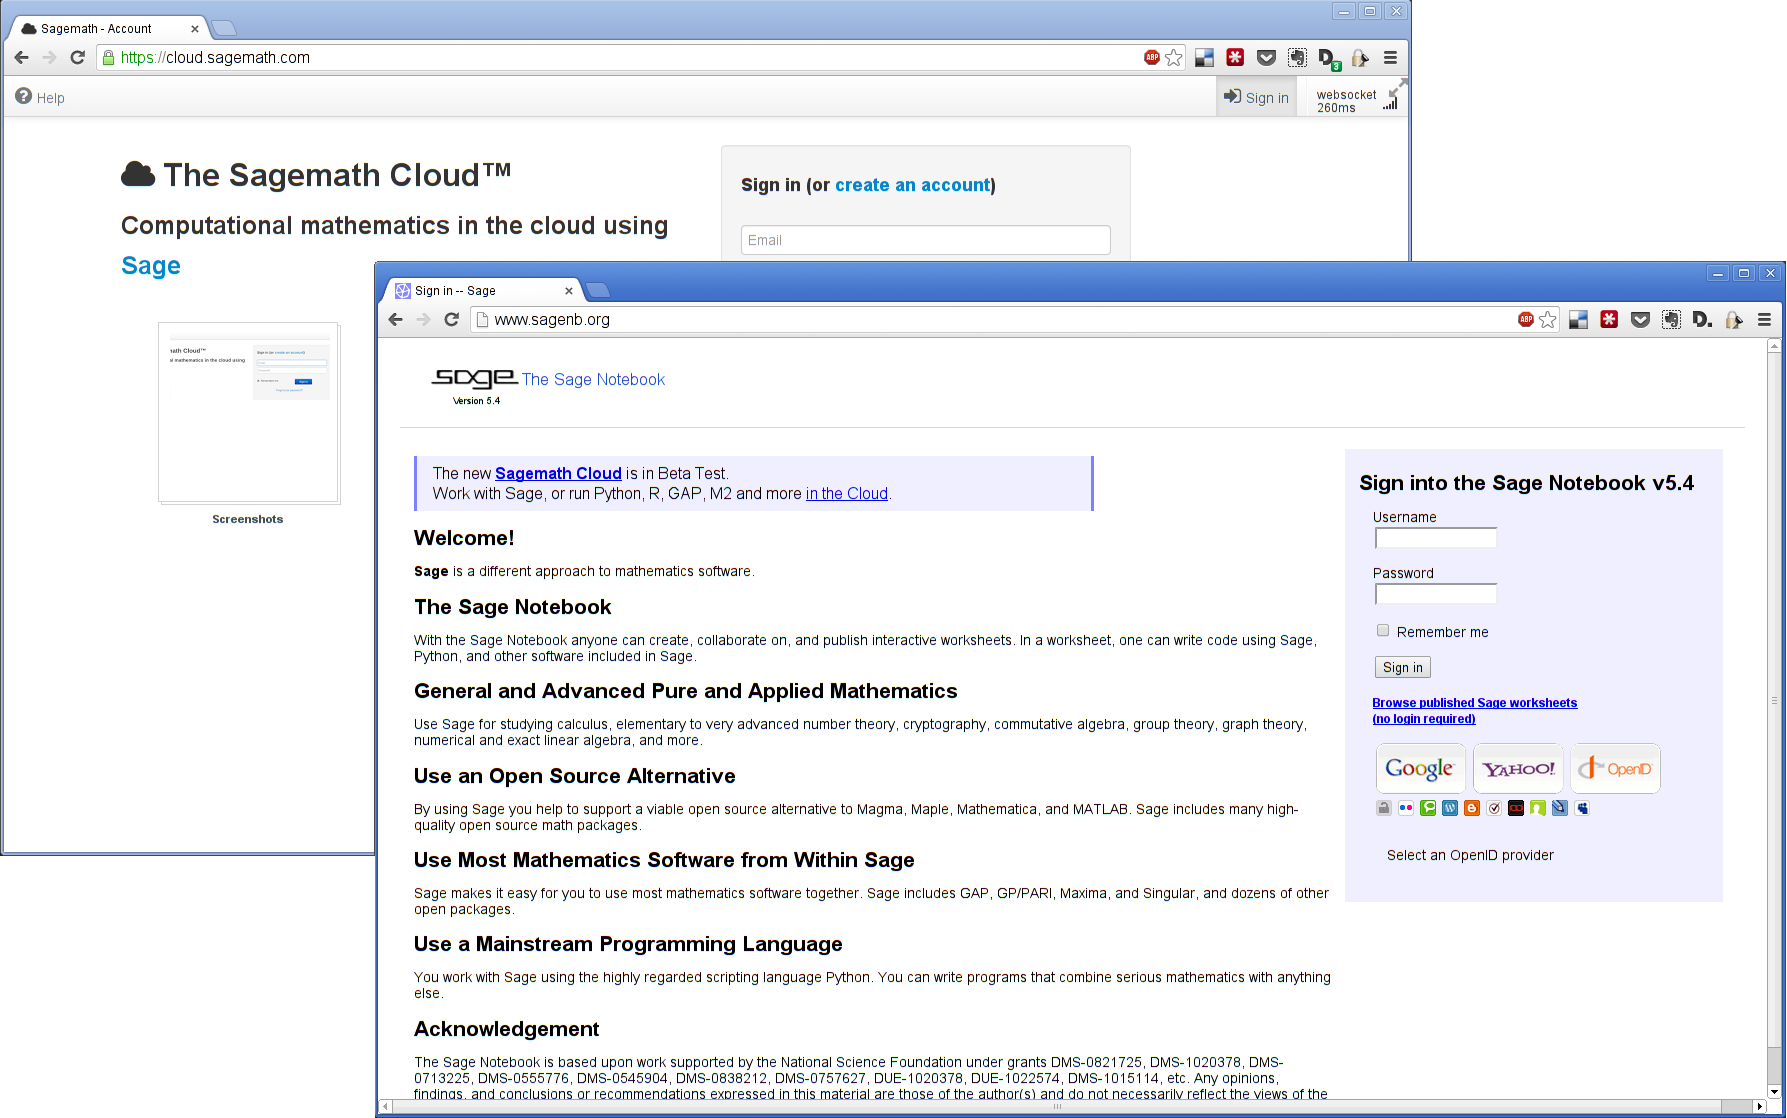
\includegraphics[width=\textwidth]{sage-online.png}
\end{center}

\framebreak

If you just want to do a quick calculation (and share it with others), try 

\begin{center}
\url{http://aleph.sagemath.org} 
\end{center}

\begin{center}
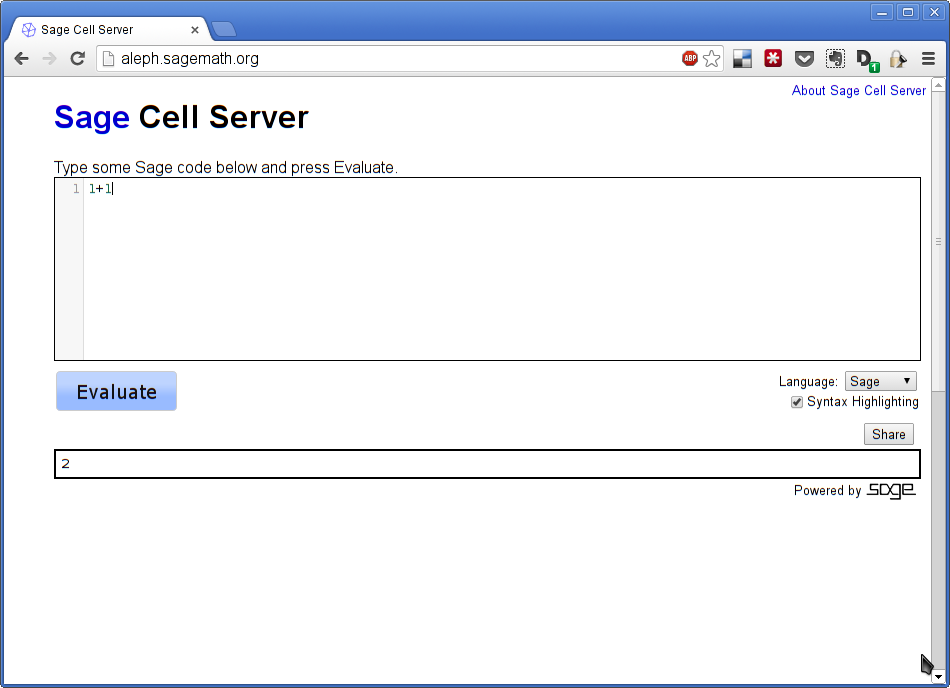
\includegraphics[width=0.7\textwidth]{sage-aleph.png}
\end{center}

\framebreak

You can access a Sage 5.10 installed on IMM servers using your account credentials.
\begin{lstlisting}[language=bash,basicstyle=\tiny\tt]
malb@road:~ $ ssh maroa@sunray4.imm.dtu.dk
Password: 
Last login: Mon Oct  7 17:20:54 2013 from 10.16.166.157
Sun Microsystems Inc.   SunOS 5.10      Generic January 2005

sunray4:~ $ gridterm
perl: warning: Setting locale failed.
perl: warning: Please check that your locale settings:
        LC_ALL = (unset),
        LC_CTYPE = "iso_8859_1",
        LANG = "en_US.utf8"
    are supported and installed on your system.
perl: warning: Falling back to the standard locale ("C").
Last login: Mon Oct  7 17:30:24 CEST 2013 from sunray4.imm.dtu.dk on pts/18

grid03:~ $ sage
+--------------------------------------------------------------------+
| Sage Version 5.10, Release Date: 2013-06-17                        |
| Type "notebook()" for the browser-based notebook interface.        |
| Type "help()" for help.                                            |
+--------------------------------------------------------------------+
sage: 1+1
2
\end{lstlisting}

\end{frame}

\begin{frame}
\frametitle{Intro to Programming in Sage} 

\begin{block}{}
Go to Sage Worksheet. 
\end{block}

\vspace{2em}

See also 

\begin{center}
\footnotesize
\url{http://sagemath.org/doc/thematic_tutorials/tutorial-programming-python.html}
\end{center}

\end{frame}


\section{Polynomial Rings}

\begin{frame}[fragile,allowframebreaks]
\frametitle{Notation}

\begin{itemize}
 \item By \F we denote any field field in which we can effectively compute, e.g.~\Q, or
 \item \F[q] is the finite field of order $q$ where $q$ is a prime power, e.g.~$\F[2^3]$ or $\F[7]$
 \item $P = \F{}[\gens]$ is the polynomial ring in \gens over \F.
 \item We assume $n$ is finite in this lecture.
\end{itemize}

\begin{lstlisting}
sage: P.<x,y,z> = PolynomialRing(FiniteField(7))
sage: f = x*y + 3*y*z -3
sage: g = x^2 - 2*y^2 
sage: f * g
x^3*y - 2*x*y^3 + 3*x^2*y*z + y^3*z - 3*x^2 - y^2
sage: f + g
x^2 + x*y - 2*y^2 + 3*y*z - 3
\end{lstlisting}

\framebreak

Let $f = 3xy + 2$, we call

\begin{description}
 \item[{\bf monomials}] $3\memph{\bf xy} + 2\cdot \memph{\bf 1}$
 \item[{\bf coefficients}] $\memph{3}xy + \memph{2}\cdot 1$
 \item[{\bf terms}] $\memph{3xy} + \memph{2}$
\end{description}

This follows \cite{cox-little-oshea:2007} and is consistent with the usage in Sage.

\begin{lstlisting}
sage: P.<x,y> = PolynomialRing(FiniteField(7))
sage: f = 2*x*y +3
sage: f.monomials()
[x*y, 1]
sage: f.coefficients()
[2, 3]
\end{lstlisting}

But \cite{becker-weispfenning:1991} swap the notion of term and monomial.

\end{frame}

\begin{frame}[allowframebreaks,fragile]
\frametitle{Monomial Orderings} 
We will have to make decisions based on the ``leading monomial'' of a polynomial, which begs the question what that is.
\begin{itemize}
\item In $\F{}[x]$ this question is straight-forward: $x^i > x^j$ iff $i>j$.
\item But what about $\F{}[x,y]$ is $x^2$ or $xy$ bigger?
\item Hence, we adjoin a \memph{monomial ordering} to our ring $\F{}[\gens]$
\end{itemize}

\framebreak

\begin{definition}[Lexicographical]
Let $$m_1 = x_1^{\alpha_1} x_2^{\alpha_2} \cdots x_n^{\alpha_n} \textnormal{ with } \alpha = (\alpha_1,\dots,\alpha_n)$$ and $$m_2 =  x_1^{\beta_1} x_2^{\beta_2} \cdots x_n^{\beta_n} \textnormal{ with } \beta = (\beta_1,\dots,\beta_n).$$  We say $m_1 >_{\textrm{lex}} m_2$ if, in the vector difference $\alpha - \beta \in \Z^n$, the leftmost nozero entry is positive.
\end{definition}

Like in the dictionary: first you check  $x$, then $y$ \dots.

$$(0,5,3) - (0,2,9) = (0,3,-6) \Rightarrow y^5z^3 >_{\textrm{lex}} y^2z^9 \in \F{}[x,y,z]$$

\framebreak

\begin{definition}[Degree Lexicographical]
Let $$m_1 = x_1^{\alpha_1} x_2^{\alpha_2} \cdots x_n^{\alpha_n} \textnormal{ with } \alpha = (\alpha_1,\dots,\alpha_n)$$ and $$m_2 =  x_1^{\beta_1} x_2^{\beta_2} \cdots x_n^{\beta_n} \textnormal{ with } \beta = (\beta_1,\dots,\beta_n).$$  We say $m_1 >_{\textrm{deglex}} m_2$ if, $$|\alpha|  = \sum_{i=1}^{n} \alpha_i > |\beta| = \sum_{i=1}^{n} \beta_i \textnormal{, or } |\alpha| = |\beta| \textnormal{ and } \alpha >_{\textrm{lex}} \beta.$$
\end{definition}

We first check for degrees and only if those are equal we compare lexicographically.

$$y^2z^9 >_{\textrm{deglex}} y^5z^3 \in \F{}[x,y,z]$$

\framebreak

\begin{definition}[Degree Reverse Lexicographical]
Let $$m_1 = x_1^{\alpha_1} x_2^{\alpha_2} \cdots x_n^{\alpha_n} \textnormal{ with } \alpha = (\alpha_1,\dots,\alpha_n)$$ and $$m_2 =  x_1^{\beta_1} x_2^{\beta_2} \cdots x_n^{\beta_n} \textnormal{ with } \beta = (\beta_1,\dots,\beta_n).$$ We say $m_1 >_{\textrm{degrevlex}} m_2$ if, $$|\alpha|  = \sum_{i=1}^{n} \alpha_i > |\beta| = \sum_{i=1}^{n} \beta_i \textnormal{, or }$$ $|\alpha| = |\beta|$ and the rightmost nonzero entry of $\alpha - \beta \in \Z^n$ is negative.
\end{definition}

$>_{\textrm{deglex}}$ is not $>_{\textrm{degrevlex}}$ with reversed variables:

$$x^2yz^2 >\not>_{\textrm{degrevlex}} xy^3z\ \textnormal{ vs. }\ x^2yz^2 >_{\textrm{deglex}} xy^3z.$$

\framebreak

\begin{lstlisting}
sage: P.<x,y,z> = PolynomialRing(FiniteField(7), order="lex")
sage: x^2*y*z^2 > x*y^3*z
True

sage: P.<x,y,z> = PolynomialRing(FiniteField(7), order="deglex")
sage: x^2*y*z^2 > x*y^3*z
True

sage: P.<x,y,z> = PolynomialRing(FiniteField(7), order="degrevlex")
sage: x^2*y*z^2 > x*y^3*z                                 
False
\end{lstlisting}

\framebreak

\begin{itemize}
\item We write $>$ for any monomial ordering (such as $>_{\textrm{lex}}$) when it is clear from context which we mean
\item \LM{f}: We call leading monomial of $f$ that monomial in $f$ which is largest wrt to $>$.
\item \LC{f}, \LT{f}: We define the leading coefficient  and leading term  of $f$ analogously.
\item We extend the notion of $>$ to polynomials $f,g$ in the natural way by comparing $\LM{f}$ and $\LM{g}$ first and move on to smaller monomials if they are equal.
\item $\deg(f)$: We call the degree of $f$ the maximal degree of any monomial in $f$. In particular, $\deg(f)$ can be $\neq \deg(\LM{f})$.
\end{itemize}
\end{frame}

\begin{frame}
\frametitle{Exercises}
\begin{itemize}
\item Construct $\F[7][x,y,z]$ with term order \memph{deglex} in Sage
\item Reorder the monomials of $f = 4 x^{5} y z^{4} + 2 x^{2} y^{8} -  x y^{4} + x y z^{3} + 4 y z + 3 x$ wrt to the
\begin{itemize}
    \item \memph{lexicographical},
    \item \memph{degree lexicographical} and
    \item \memph{degree reverse lexicographical}
\end{itemize}
 ordering. Check your result with Sage.
\end{itemize}
\end{frame}


\begin{frame}[allowframebreaks,fragile]
\frametitle{Polynomial Division} 

We will need to divide polynomials (with remainder) later:

\vspace{1em}

Division of monomials is easy: $x_1^{\alpha_1} \cdots x_n^{\alpha_n}$ is divisible by $x_1^{\beta_1} \cdots x_n^{\beta_n}$ if $\alpha - \beta \geq (0,\dots,0)$ where $\alpha = (\alpha_1,\dots,\alpha_n)$ and $\beta = (\beta_1,\dots,\beta_n)$.

\vspace{1em}

But what about polynomials?

\framebreak

\begin{columns}
\column{0.55\textwidth}
\begin{algorithm}[H]
\SetKw{KwAnd}{and}
\SetKw{KwOr}{or}
\SetKw{KwBreak}{break}
\Begin{
$a_1,\dots,a_s \gets 0,\dots,0$;\ \ $r \gets 0$\;
\While{$p \neq 0$\nllabel{div:while}}{
  division $\gets$ False\;
  \For{$1 \leq i \leq s$}{
      \If{$\LM{f_i}$ divides $\LM{p}$}{
        $a_i \gets a_i + \LT{p}/\LT{f_i}$\;
        $p \gets p - \LT{p}/\LT{f_i}\cdot f_i$\;
        division $\gets$ True\;
        \KwBreak;
      }   
  }
  \If{division = False}{
    $r \gets r + \LT{p}$\;
    $p \gets p - \LT{p}$\;
  }
}
}
\caption{Polynomial Division}
\end{algorithm}
\column{0.45\textwidth}
\begin{example}
$p = 3x^2y + 2y^2 + x + 1$,\\
$f_1 = 2x^2 + 1$, \\
$f_2 = y + 1 \in \F[7][x,y]$ with deglex\\

\begin{enumerate}
 \item $x^2 \mid x^2y:$\\$a_1 = -2y$, $p = 2y^2 + x + 2y + 1$
 \item break and jump to line~\ref{div:while}.
 \item $y \mid y^2:$\\$a_2 = 2y$, $p = x + 1$
 \item break and jump to line~\ref{div:while}.
 \item Neither $y$ nor $x^2$ divide $x$: division = False
 \item $r = x$, $p = 1$
 \item Neither $y$ nor $x^2$ divide $x$: division = False
 \item $r = x + 1$, $p = 0$
\end{enumerate}
\end{example}
\end{columns}

\framebreak

\begin{lstlisting}
sage: P.<x,y> = PolynomialRing(FiniteField(7),order="deglex")      
sage: f = 3*x^2*y + 2*y^2 + x + 1
sage: f1 = 2*x^2 + 1
sage: f2 = y + 1
sage: f == (-2*y)*f1 + (2*y)*f2 + (x+1)
True
\end{lstlisting}

\end{frame}

\begin{frame}
\frametitle{Exercises}
\begin{itemize}
\item Let $f = x^7y^2 + x^3y^2 - y + 1$, $f_1 = xy^2 - x$ and $f_2 = x-y^3 \in \F[7][x,y]$ with \memph{deglex}. Divide $f$ by $(f_1,f_2)$. Then use \memph{lex} and divde again.

\item Let $f = xy^2 - x$, $f_1 = xy + 1$ and $f_2 = y^2 -1 \in \F[7][x,y]$ with $>_{\textrm{lex}}$.\\
Divide $f$ by $(f_1,f_2)$ and by $(f_2,f_1)$ and compare the remainders.

\item Let $f = xy^2z^2 + xy - yz$, $f_1 = x - y^2$, $f_2 = y-z^3$ and $f_3 = z^2 -1 \in \F[7][x,y,z]$ with \memph{deglex}.\\
Divide $f$ by $(f_1,f_2,f_3), (f_2,f_3,f_1)$ and $(f_3,f_1,f_2)$ and compare the remainders.
\end{itemize}
\end{frame}


\section{Ideals}

\begin{frame}[fragile]
\frametitle{Definition}
Let $\I$ be an ideal $ \subset P$. 

\vspace{1em}

That is,
\begin{itemize}
 \item $0 \in \I$,
 \item If $f,g \in \I$, then $f + g \in \I$, and 
 \item if $f \in P, g \in \I$, then $f \cdot g \in \I.$
\end{itemize}

We denote by $\ideal{f_1,\dots,f_s}$ is the ideal spanned by $f_1,\dots,f_s$, i.e.\ all
$$f = a_1f_1 + \cdots +a_sf_s.$$

\begin{lstlisting}
sage: P.<x,y,z> = PolynomialRing(FiniteField(127),order='deglex')
sage: I = ideal(x*y + z, y^3 + 1, z^2 - x*5 - 1)
sage: (x*y + z) + (y^3 + 1) in I
True
sage: x*z*(z^2 - x*5 - 1) in I
True
\end{lstlisting}
\end{frame} 


\begin{frame}[allowframebreaks,fragile]
\frametitle{Varieties}
\begin{definition}
Let \F{} be a field, and let $f_1,\dots , f_s$ be polynomials in $\F{}[\gens]$. Then we set
$$V(f_1, \dots, f_s) = \{(a_1, \dots , a_n) \in \F{}^n : f_i(a_1, \dots , a_n) = 0 \textnormal{ for all } 1 ≤ i ≤ s\}.$$
We call $V(f_1, \dots, f_s)$ the affine variety defined by $f_1,\dots, f_s$.
 
\end{definition}

\vspace{1em}

It's the set of all solutions to $f_i(\gens) = 0$ for all $1 \leq i \leq s$.

\vspace{1em}

For example, $f_1 = x^2 + y^2 - 1 \in \mathbb{R}[x,y]$ is the unit circle.

\framebreak

\begin{block}{Lemma}
$V(\I)$ is an affine variety. In particular, if $\I= \ideal{ f_1, \dots, f_m}$, then $V(\I) = V(f_1, \dots, f_m)$.
\end{block}
 
\begin{block}{Corollary}
If $f_1, \dots , f_s$ and $g_1, \dots , g_t$ are bases of the same ideal in $\F{}[\gens]$, so that $\ideal{f_1,\dots, f_s} = \ideal{g_1,\dots, g_t}$, then we have $V(f_1 ,\dots , f_s) =
V(g_1, \dots , g_t)$.
\end{block}

\vspace{1em}

\dots so finding a good basis $g_1,\dots,g_t$ for $\ideal{f_1,\dots,f_s}$ such that finding $V(f_1,\dots,f_s) = (g_1,\dots,g_t)$ is easy would allow to solve non-linear systems of equations.

\framebreak

\begin{example}{}
Consider $\I = \ideal{x^2 + y^2 -1, xy} \in \F[7][x,y]$. The set of all points satisfying all polynomials in $\I$ are $(0, 1), (0, -1), (1, 0), (-1, 0)$.
\end{example}

\vspace{1em}

The same in Sage:

\begin{lstlisting}
sage: P.<x,y> = PolynomialRing(FiniteField(7))
sage: I = Ideal(x^2 + y^2 - 1, x*y)
sage: I.variety()
[{y: 0, x: 1}, {y: 0, x: 6}, {y: 1, x: 0}, {y: 6, x: 0}]
\end{lstlisting}


\end{frame}


\begin{frame}
\frametitle{Exercises}
\begin{enumerate}
 \item Construct the Ideal $\I = \ideal{xy +1, y^2 -1} \in \F[7][x,y]$ in Sage with monomial ordering \memph{deglex}.
 \item Show that $x+y \in \I$.
 \item Is $\{1\}$ an ideal? Is $\{x + 1, y -2\}$ an ideal?
 \item Show that $\ideal{1}$ and $\ideal{x+1,x-1,y-2}$ are the same.
 \item What is $V(\{1\})$? 
 \item What is $V(\ideal{x+1, y-1})$?
 \item What is $V(x+y, x+1)$?
\end{enumerate}
 

\end{frame}

\section{Gröbner Bases}

\begin{frame}[allowframebreaks,fragile]
\frametitle{Definition}
\begin{definition}[Gr\"obner Basis]
Let $\I$ be an ideal in $\F{}[\gens]$ and fix a monomial ordering. A finite subset $$G = \{g_1 ,\dots , g_{m} \} \subset \I$$  is said to be a \textbf{Gr\"obner basis} of $\I$ if for any $f \in \I$ there exists $g_i \in G$ such that $$\LM{g_i} \mid \LM{f}.$$
\end{definition} 

\framebreak

Gröbner bases generalise greatest common divisors over $\F{}[x]$: the GCD divides all its multiples.

\begin{lstlisting}
sage: R.<x> = PolynomialRing(FiniteField(7))
sage: f = x^2 + 6
sage: I = Ideal(map(P, [R.random_element() * f for _ in range(5)]))
sage: I.groebner_basis()
[x^2 - 1]
\end{lstlisting}

\framebreak

\dots and row echelon forms over $\F{}^n$: if $y + tail$ is in the vector space, the row echelon form has an element $y + tail'$. 
\begin{lstlisting}
sage: F = Sequence([-3*y, -2*x - y - 3*z + 2, x + y + 2*z - 1])
sage: F.groebner_basis()
[x - 1, y, z]
sage: A,v = F.coefficient_matrix()
sage: A.echelonize()
sage: (A*v).T
[x - 1     y     z]
\end{lstlisting}

\framebreak

You can use Sage to check if a list of polynomials is a Gröbner basis:

\begin{lstlisting}
sage: P.<x,y,z> = PolynomialRing(FiniteField(7),order="degrevlex")
sage: I = Ideal([x*y^2 - z, 2*x^2*y - 2, x*y - z + 1])
sage: I.basis_is_groebner()
False

sage: I.groebner_basis()
[y^2 - y - z + 1, y*z - y - z, z^2 - y - 2*z + 1, x - y + 1]
\end{lstlisting}


\end{frame}


\begin{frame}[allowframebreaks,fragile]
\frametitle{Reduced Gröbner Bases} 

\begin{definition}[Reduced Gröbner Basis]
A \textbf{reduced Gröbner basis} for a polynomial ideal $\I$ is a
Gröbner basis $G$ such that:
\begin{enumerate}
\item $\LC{f} = 1$ for all $f \in G$;
\item $\forall f \in G, \not\exists\ m \in $\ the set of monomials of $f$ such that $m$ is divisible by any $\LM{g} \in G \setminus \{f\}$.
\end{enumerate}
\end{definition}

\vspace{1em}
Reduced Gröbner bases generalise reduced row echelon forms:

\[
\left(\begin{array}{rrrrrrrr}
2 & 4 & 5 & 6 & 3 & 5 & 2 & 5 \\
  & 5 & 2 & 2 & 2 & 1 & 0 & 2 \\
  &   & 6 & 5 & 6 & 2 & 1 & 6 \\
  &   &   & 2 & 3 & 6 & 4 & 0 \\
  &   &   &   & 3 & 0 & 3 & 1 \\
  &   &   &   &   &   & 1 & 6
\end{array}\right)
\Rightarrow 
\left(\begin{array}{rrrrrrrr}
1 & 0 & 0 & 0 & 0 & 0 & 0 & 1 \\
  & 1 & 0 & 0 & 0 & 5 & 0 & 6 \\
  &   & 1 & 0 & 0 & 6 & 0 & 1 \\
  &   &   & 1 & 0 & 3 & 0 & 0 \\
  &   &   &   & 1 & 0 & 0 & 6 \\
  &   &   &   &   &   & 1 & 6
\end{array}\right)
\]

\framebreak

\framebreak

By default, Sage will always computes the reduced Gröbner basis when computing a Gröbner basis. If a Gröbner basis was obtained by other means, the function 
\begin{lstlisting}
MPolynomialIdeal.interreduced_basis()
\end{lstlisting}
can be used to compute the reduced Gröbner basis.
\begin{lstlisting}
sage: rgb = Ideal(gb).interreduced_basis()
\end{lstlisting}

\end{frame}

\begin{frame}[fragile,allowframebreaks]
\frametitle{Applications}
\begin{description}
 \item[\bf Representation] Reduced Gröbner bases are a unique representation of an ideal with respect to a monomial ordering. So to check that two ideals are the same you only need to compute their reduced Gröbner bases.

\begin{lstlisting}
sage: P.<x,y,z> = PolynomialRing(FiniteField(7))
sage: I = Ideal(P.random_element() for _ in range(5))
sage: J = Ideal(P.random_element() for _ in range(5))
sage: I = Ideal(f - f((2,3,1)) for f in I.gens())
sage: J = Ideal(f - f((2,3,1)) for f in J.gens())
sage: I.groebner_basis() == J.groebner_basis()
True
sage: I == J
True
sage: I.gens() == J.gens()
False 
sage: I.groebner_basis()
[x - 2, y - 3, z - 1]
\end{lstlisting}

\framebreak

 \item[\bf Membership] The remainder $r$ of the division of any $f \in P$ by $G$ is unique. Hence, we can check whether $f \in \ideal{f_1,\dots,f_s}$ by computing a Gröbner basis $G = (g_1,\dots,g_t)$ for $\ideal{f_1,\dots,f_s}$ and check if $\overline{f}^G = 0$.

\begin{lstlisting}
sage: P.<x,y,z> = PolynomialRing(FiniteField(7))
sage: I = Ideal(P.random_element() for _ in range(5))
sage: I = Ideal(f - f((2,3,1)) for f in I.gens())

sage: f = P.random_element()
sage: f in I
False

sage: f = f - f((2,3,1))
sage: f in I
True

sage: f.reduce(I.gens())
2*z^2 + y - 3*z - 2
sage: f.reduce(I.groebner_basis())
0
\end{lstlisting}

\framebreak

\item[\bf Solving] Gröbner bases with respect to the \memph{lex} ordering allow for finding $V(\I)$ easily. We can ``read off'' the solution similarly to reading the solution from a row echelon form of a matrix.

\begin{lstlisting}
sage: P.<x,y,z> = PolynomialRing(FiniteField(7), order="lex")
sage: I = Ideal(P.random_element() for _ in range(5))
sage: I = Ideal(f - f((2,3,1)) for f in I.gens())
sage: I.groebner_basis()
[x - 2, y - 3, z - 1]
\end{lstlisting}

\end{description}

\end{frame}

\begin{frame}
\frametitle{Exercises}
 
\begin{itemize}
 \item Let $f_1,\dots,f_m$ be polynomials in $\F{}[\gens]$. Assume that $V(f_1,\dots,f_m) = \{(s_1,\dots,s_n)\}$. Show that the reduced Gröbner basis of $\I = \ideal{f_1,\dots,f_m}$ is $[x_1 - s_1, \dots, x_n - s_n]$.
 \item If we use \memph{degrevlex} order with $x > y > z$, is \[\{x^4 y^2 - z^5 , x^3 y^3 − 1, x^2 y^4 − 2z\}\] a Gröbner basis or the ideal generated by these polynomials? Why or why not?
 \item $\{x + 1, y - 2, xy - 2x + y - 2\}$ is a Gröbner basis wrt the \memph{degrevlex} ordering in $\F[7][x,y]$. Is it a reduced Gröbner basis? Is $\{2x + 2, 3y + 1\}$? If not, why not?
\end{itemize}


\end{frame}

\section{Buchberger's Algorithm}


\begin{frame}[allowframebreaks,fragile]
\frametitle{S-Polynomials}

Let $G = \{f_1,\dots,f_s\} \subset \F{}[\gens]$ and $\I = \ideal{G}$. If there exists any $f \in \I$ with $$\LM{f} \textnormal{ is not divisible by any } \LM{f_1}, \dots,\LM{f_m},$$ then $G$ is not a Gröbner basis for $\ideal{G}$; by definition.

\framebreak

To obtain a candidate for such $f$ from $f_1,\dots,f_s$, we may choose two elements $f_i$ and $f_j$ of $G$ and compute \[s = ax^\alpha f_i - bx^\beta f_j \textnormal{ with } a,b \in \F{}.\]
We know that $\LM{ax^\alpha f_i - bx^\beta f_j}$ is divisible by an element of the Gröbner basis of $\I$ because $ax^\alpha f_i - bx^\beta f_j \in \I$. 

\framebreak

Now assume that in $s$ the terms $ax^\alpha\LT{f_i}$ and $bx^\beta\LT{f_j}$ cancel each other out. 

\vspace{1em}

If as a result $\LM{ax^\alpha f_i\ -\ bx^\beta f_j}$ is not divisible by any $ \LM{f_1}, \dots ,\LM{f_t}$ we know that $G$ cannot be a Gröbner basis. 

\framebreak

S-polynomials are a (in fact: \memph{the}) way to construct the required cancellations of leading terms:


\begin{definition}[S-Polynomial]
\label{def:spolynomials}
Let $f,g \in \F{}[\gens]$ be non-zero polynomials.
\begin{enumerate}
\item Let $x^\gamma$ be the least common multiple of $\LM{f}$ and $\LM{g}$, written as $$x^\gamma = \LCM{\LM{f},\LM{g}}.$$  
\item The S-polynomial of $f$ and $g$ is defined as
\begin{align*}
S(f,g)\ =\ \frac{x^\gamma}{\LT{f}}\cdot f\ -\
\frac{x^\gamma}{\LT{g}}\cdot g.
\end{align*}
\end{enumerate}
We call $f$ and $g$ the \textbf{generators} of $S(f,g)$ and $\frac{x^\gamma}{\LT{f}}\cdot f$  and $\frac{x^\gamma}{\LT{g}}\cdot g$ the \textbf{components} of $S(f,g)$.
\end{definition}

\framebreak

\begin{example}
 Let $f_1 = x^3 - 2xy$ and $f_2 = x^2y - 2y^2 + x$. The leading monomials with respect to \memph{degrevlex} and $x > y$ are
$\LM{f_1} = x^3$ and $\LM{f_2} = x^2y$ and thus $x^\gamma = x^3y$. The S-polynomial is:
\begin{eqnarray*}
S(f_1,f_2) &=& \dfrac{x^\gamma}{\LT{f_1}} \cdot f_1 - \dfrac{x^\gamma}{\LT{f_2}} \cdot f_2\\
S(f_1,f_2) &=& \dfrac{x^3y}{x^3} \cdot (x^3 - 2xy) -\ \dfrac{x^3y}{x^2y} \cdot (x^2y - 2y^2 + x)\\
S(f_1,f_2) &=& y \cdot (x^3 - 2xy) -  x \cdot (x^2y - 2y^2 + x)\\
S(f_1,f_2) &=& x^3y - 2xy^2 -  x^3y + 2xy^2 - x^2\\
S(f_1,f_2) &=& -x^2
\end{eqnarray*}
\end{example}

\framebreak

The same example in Sage:

\begin{lstlisting}
sage: P.<x,y> = PolynomialRing(QQ,order='degrevlex')
sage: f0 = x^3 - 2*x*y
sage: f1 = x^2*y -2*y^2 + x
sage: (x^3*y)//x^3 * f0 - (x^3*y)//(x^2*y) * f1
-x^2
\end{lstlisting}

\framebreak

\begin{block}{}
It is \textbf{sufficient} to consider \textbf{only} S-polynomials since \textbf{any} reduction of leading terms can be attributed to S-polynomials. 
\end{block}

\vspace{1em}

\begin{thebibliography}{fooobaaa}
\bibitem{Buc64}[Buc65] Bruno Buchberger
\newblock Ein {A}lgorithmus zum {A}uffinden der {B}asiselemente des {R}estklassenrings nach einem nulldimensionalen {P}olynomideal,
\newblock Phd Thesis at Universität Innsbruck, 1965.

\bibitem{Buc06}[Buc06] Bruno Buchberger
\newblock Bruno Buchberger's PhD thesis 1965: An algorithm for finding the basis elements of the residue class ring of a zero dimensional polynomial ideal
\newblock Journal of Symbolic Computation, 41:3-4, p.\ 475-511, 2006.

\end{thebibliography}

\end{frame}

\begin{frame}[allowframebreaks]
\frametitle{Buchberger's Criterion}

\begin{block}{Buchberger's Criterion}
\label{theorem:buchberger}
Let $\I$ be an ideal. $G\ =\ \left\lbrace g_1,\ \dots\ ,g_{s}\right\rbrace$ is
a Gröbner basis for $\I$, if and only if for all pairs $i \neq j$, the remainder $r$ of the division of $S(g_i,g_j)$
by $G$ (listed in some order) is zero, i.e.\ we have that $\overline{f}^{G} = 0$.
\end{block}

\begin{proof}
See \cite[p.85ff]{cox-little-oshea:2007}
\end{proof}

\framebreak

\begin{example}
Let $f_1 = x^3 - 2xy$ and $f_2 = x^2y - 2y^2 + x$. The S-polynomial is $-x^2$ which is not reducible by either $\LM{f_1} = x^3$ or $\LM{f_2} = x^2y$. Thus, $(f_1,f_2)$ is not a Gröbner basis.
\end{example}

\end{frame}


\begin{frame}[fragile]
\frametitle{Buchberger's Algorithm}

\begin{columns}
 
\column{0.55\textwidth}
 
\begin{algorithm}[H]
\KwIn{$F$ -- a finite subset of $P$}
\KwResult{a Gröbner basis for the ideal $\I$ spanned by $F$}

\Begin{
$G \longleftarrow F$\;
$G_2 \longleftarrow \varnothing$\;
\While{$G_2 \neq G$}{
  $G_2 \longleftarrow G$\;
  \For{$f,g \in G_2 \times G_2$}{
      \If{$\LM{f}<\LM{g}$}{
       $ \tilde{s} \longleftarrow \overline{S(f,g)}^G$\;
       \If{$\tilde{s}\neq 0$}{add $\tilde{s}$ to $G$\;}
      }
   }
 }
 \Return{G}\;
}
\caption{Buchberger's Algorithm}
\label{alg:buchberger}
\end{algorithm}

\column{0.45\textwidth}

Correctness and termination:
\begin{enumerate}
\item At every stage of the algorithm, $G \subset \I$ and $\ideal{ G } = \I$ hold.
\item If $G_2 = G$ then $\overline{S(f, g)}^G = 0$ for all $f, g \in G$ and, by Buchberger's criterion, $G$ is a Gröbner basis.
\item The equality $G_2 = G$ occurs in finitely many steps since the ideals $\ideal{\LM{G}}$, in iterations of the loop, form an ascending chain. This chain of ideals stabilizes after a finite number of iterations and at that moment $\ideal{\LM{G}} = \ideal{\LM{G_2}}$ holds, which implies $G_2 = G$.
\end{enumerate}

\end{columns}
\end{frame}

\begin{frame}
\frametitle{Complexity}

The running time of Buchberger's algorithm is not polynomial in the number of variables, as the intermediate bases $G_2$ grow exponentially during the calculations.

\begin{block}{Theorem~\cite{faugere-ars:inria2004}}
Let $\I$ be an ideal in $\F[q][\gens]$ generated by polynomials $f_1,\dots,f_n$ of degrees $d_1,\dots,d_n$ respectively. Assume $V(\I)$ is finite.
\begin{itemize}
 \item A Gröbner basis computation for a \textbf{lex} monomial order reaches at most degree $D \leq \prod_{i=0}^{n-1} d_i$.
 \item A Gröbner basis computation for a \textbf{degrevlex} monomial order reaches at most degree $D \leq 1 - n + \sum_{i=0}^{n-1} d_i$.
\end{itemize}
\end{block}
\end{frame}

\begin{frame}[allowframebreaks]
\frametitle{Optional Improvements}
Buchberger's algorithm leaves a lot of freedom to implement. The runtime can be reduced by applying a variety of improvements:
\begin{itemize}
\item The order in which the critical pairs $f,g$  are selected.
\item If $\overline{S(f,g)}^G = 0$ we learn nothing new, we can employ criteria to filter out such computations.
\item Algorithms exist \cite{faugere-gianni-lazard-mora:joc1993} to convert a Gröbner basis (of an ideal with $V(\I)$ finite) in one monomial order to a Gröbner basis in another monomial order, thus we may compute with respect to the \memph{degrevlex} ordering first and then convert the result to \memph{lex}.
\end{itemize}

\framebreak

Buchberger himself gave two criteria to avoid useless reductions to zero. We only give the first one here:

\begin{definition}[Buchberger's First Criterion]
Let $f,g \in \F{}[\gens]$ with disjoint leading terms, i.e.\ $\LCM{\LM{f},\LM{g}} = \LM{f}\cdot\LM{g}$. Then $\overline{S(f,g)}^G = 0$.
\label{def:buchberger_first_criterion}
\end{definition}

\begin{proof}
See \cite[p.222]{becker-weispfenning:1991}. 
\end{proof}

\end{frame}

\begin{frame}
\frametitle{Exercises}

\begin{enumerate}
 \item In $\F[7][x,y]$ with \memph{deglex} compute a Gröbner basis for $$\ideal{x^{2} y + 6, x y^{2} -  x}$$ using Buchberger's algorithm. How many reductions to zero $\overline{S(f,g)}^G = 0$ did you observe?
\item Repeate Exercise 1 in $\F[7][x,y,z]$ with \memph{deglex} for $$\ideal{x^{2} + y, x^{4} + 2 x^{2} y + y^{2} + 3}$$ what does the result tell you abour $V(\I)$?
\item Repeate Exercise 2 with $$\ideal{x - z^4, y - z^5}$$ and use Buchberger's First Criterion to avoid useless reductions to zero. How many did you avoid?
\end{enumerate}
 
\end{frame}

\section{Quotient Rings}

\begin{frame}[allowframebreaks]
\frametitle{Quotient Rings}

\begin{itemize}
 \item Recall that we considered finite extension fields as $\F[p][x]/f(x)$ for some irreducible polynomial $f(x)$.
 \item By this we mean that all multiplies  of $f(x)$ are zero, i.e., we quotient out by elements in $\ideal{f(x)}$.
 \item In fact, we can quotient out by any ideal $\I$ and define the quotient ring $Q = R/\I$.
\end{itemize}


\begin{block}{Theorem~\cite[p.226]{cox-little-oshea:2007}}
Let $\I$ be an ideal in $\F[][\gens]$. The ideals in the quotient ring $\F[][\gens]/\I$ are in one-to-one
correspondence with the ideals in $\F[][\gens]$ containing $\I$ (that is, the ideals $\mathcal{J}$ satisfying $\I \subset \mathcal{J} \subset P$).
\end{block}

In particular, we may identify \[\I = \ideal{f_1,\dots,f_m,x_1^q - x_1,\dots,x_{n}^q-x_{n}} \in \F[q][x_1,\dots,x_{n}]\] with \[\mathcal{J} = \ideal{f_1,\dots,f_m} \in \F[q][x_1,\dots,x_{n}]/\ideal{x_1^q - x_1,\dots,x_{n}^q-x_{n}}.\]

\end{frame}

\begin{frame}[fragile]
\frametitle{Sage}

\begin{lstlisting}
sage: P.<x,y,z> = PolynomialRing(FiniteField(2))
sage: I = sage.rings.ideal.FieldIdeal(P)
sage: Q = P.quotient_ring(I); Q
Quotient of Multivariate Polynomial Ring in x, y, z \
      over Finite Field of size 2 by the ideal (x^2 + x, y^2 + y, z^2 + z)

sage: P.<x,y,z> = BooleanPolynomialRing() # much faster!
sage: P.defining_ideal()
Ideal (x^2 + x, y^2 + y, z^2 + z) of Multivariate Polynomial Ring \
      in x, y, z over Finite Field of size 2
\end{lstlisting}


\end{frame}


\section{Solving Polynomial Systems with Gröbner Bases}
\label{sec:solvingmq}

\begin{frame}[allowframebreaks,fragile]
\frametitle{Elimination Ideals}


Given an ideal $\I$ in a polynomial ring $P = \F{}[\gens]$ over a field $\F$ and a number $j \in \{1,\dots , n\}$, consider the set of all polynomials in $\I$ which involve only the variables $x_{j} ,\dots , x_{n}$. This set $I \cap \F{}[x_{j} , \dots , x_{n} ]$ is an ideal in $\F{}[x_{j},\dots,x_{n}]$.

\framebreak

\begin{definition}[Elimination Ideal]
\label{def:elimination-ideal}
Given $\I = \ideal{ f_1 ,\dots , f_m } \subset \F{}[\gens]$, the $\ell$-th elimination ideal $I_\ell$ is the ideal of $\F[x_{l} , \dots , x_n]$ defined by
\[ \I_\ell = \I \cap \F{}[x_{l} , \dots , x_{n} ].\]
\end{definition}

\framebreak

If we could compute Gröbner bases for these elimination ideals, we could start with $n=\ell$ to get a univariate polynomial. We could then factor it and substitute, which again would produce a univariate polynomial but this time in $x_{n-1}$ etc.
\end{frame}

\begin{frame}[allowframebreaks,fragile]
\frametitle{Preprocessing}

In what follows we augment our ideal in $\F[q][\gens]$ with polynomials $x_1^q - x_1,\dots,x_n^q - x_n$ which we call field polynomials. 

\vspace{1em}

That is $\I = \I \cup \{x_i^q - x_i \mid 1 \leq i \leq n\}$, which makes sure,
\begin{itemize}
 \item that our ideal has only finitely many points in $V(\I)$ and
 \item that our ideal is ``radical''.
\end{itemize}

Both of these conditions are needed for what follows.
\end{frame}

\begin{frame}[allowframebreaks,fragile]
\frametitle{Elimination Theorem}

\begin{block}{Elimination Theorem}
Let $I \subset \F{}[x_1,\dots,x_n]$ be an ideal and let $G$ be a Gröbner basis of $\I$ with respect to the \textbf{lex} monomial ordering where $x_1 > x_2 > \dots > x_n$. Then for every $1 \leq \ell \leq n$, the set 
$$G_\ell = G \cap \F{}[x_\ell,\dots,x_n]$$
is a Gröbner basis fo the $\ell$-th elimination ideal $I_\ell$. 
\end{block}

In other words, the Gröbner basis $G$ has triangular shape, which we can use to solve.

\framebreak

\begin{example}
Let $P = \F[127][x,y,z]$, the monomial ordering \textbf{lex} and consider the ideal
\begin{align*}
I = \ideal{ x + y + z, x y + x z + y z, x y z - 1}
\end{align*}
We add the field polynomials and compute the reduced Gröbner basis:
\begin{align*}
x + y + z, y^2 + yz + z^2, z^3 - 1,
\end{align*}
which has a triangular shape as predicted by the Elimination Theorem.
\end{example}

\framebreak

This result can be computed using Sage as follows:

\begin{lstlisting}
sage: P.<x,y,z> = PolynomialRing(FiniteField(127),order='lex')
sage: I = sage.rings.ideal.Cyclic(P)
sage: I
Ideal (x + y + z, x*y + x*z + y*z, x*y*z - 1) of \
Multivariate Polynomial Ring in x, y, z over \
Finite Field of size 127
sage: J = I + sage.rings.ideal.FieldIdeal(P)
sage: g0,g1,g2 = J.groebner_basis(); g0,g1,g2
(x + y + z, y^2 + y*z + z^2, z^3 - 1)

sage: factor(g2)
(z - 19) * (z - 1) * (z + 20)

sage: factor(g1(x,y,19))
(y - 1) * (y + 20)

sage: factor(g0(x,1,19))
x + 20

sage: all(f(107,1,19)==0 for f in I.gens())
True
sage: J.variety()
[{y: 19, z: 1, x: 107}, {y: 107, z: 1, x: 19}, 
 {y: 1, z: 19, x: 107}, {y: 107, z: 19, x: 1}, 
 {y: 1, z: 107, x: 19}, {y: 19, z: 107, x: 1}]
\end{lstlisting}

\end{frame}

\begin{frame}[fragile, allowframebreaks]
\frametitle{An Example}

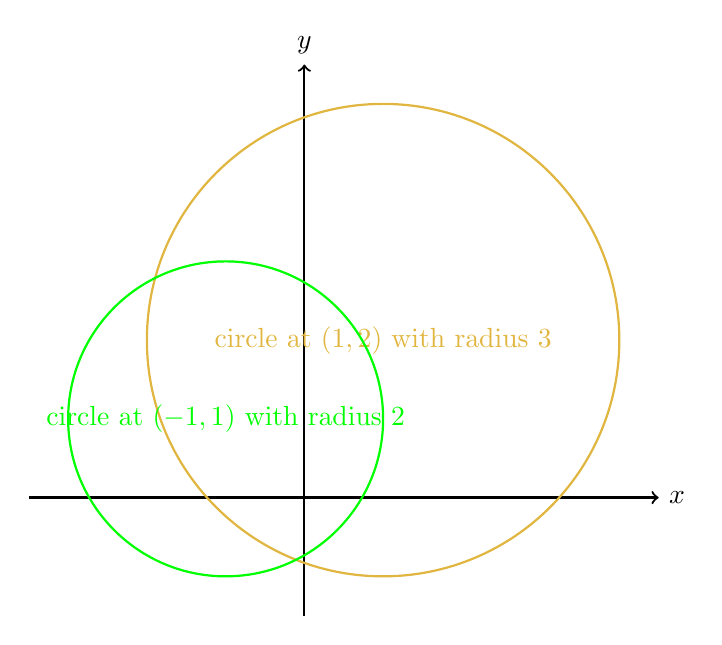
\begin{tikzpicture}
\draw [thick,->] (-3.5, 0) -- (4.5, 0) node [right] {$x$};
\draw [thick,->] (0,-1.5) -- (0, 5.5) node [above] {$y$};
\draw [yellow9,thick] (1,2) circle [radius=3] node {circle at $(1,2)$ with radius $3$};
\draw [green, thick] (-1,1) circle [radius=2]  node {circle at $(-1,1)$ with radius $2$};
\end{tikzpicture}
 
\framebreak

\begin{lstlisting}
sage: x,y = var("x, y")
sage: p1 = (x-1)^2 + (y-2)^2 - 3^2 == 0
sage: p2 = (x+1)^2 + (y-1)^2 - 2^2 == 0
sage: sols = solve([p1,p2],x,y)
sage: sols
[x == -2/5*sqrt(5) - 1, y == 4/5*sqrt(5) + 1], 
[x == 2/5*sqrt(5) - 1, y == -4/5*sqrt(5) + 1]] 
\end{lstlisting}

\framebreak

\begin{lstlisting}
sage: P.<x,y> = PolynomialRing(QQ, order='lex')
sage: f1 = (x-1)^2 + (y-2)^2 - 3^2
sage: f2 = (x+1)^2 + (y-1)^2 - 2^2 
sage: I = Ideal(f1,f2)
sage: I.groebner_basis()
[x + 1/2*y + 1/2, y^2 - 2*y - 11/5]

sage: I.variety()
[]

sage: I.variety(CC)
[{y: -0.788854381999832, x: -0.105572809000084},
  {y: 2.788854381999830, x: -1.89442719099992}]

sage: sage: P.<z> = QQ[]
sage: I.variety(NumberField(z^2-5,'a'))
[{y: -4/5*a + 1, x: 2/5*a - 1}, 
 {y: 4/5*a + 1, x: -2/5*a - 1}]
\end{lstlisting}


\end{frame}


\section{The \texorpdfstring{$\mathrm{F}_4$}{F4} Algorithm}

\begin{frame}
\frametitle{Warm Up}

As a warm-up, consider a linear system of equations over $\F[127][x,y,z]$.

\begin{columns}
\column{0.5\textwidth}
\begin{align*}
f &= 26y + 52z + 62 = 0\\
g &= 54y + 119z + 55 = 0\\
h &= 41x + 91z + 13 = 0
\end{align*}
\ After Gaussian elimination:
\begin{align*}
f' &= x + 29 = 0\\
g' &= y + 38 = 0\\
h' &= z + 75 = 0
\end{align*}
\column{0.5\textwidth}
\begin{align*}
\left(\begin{array}{rrrr}
0 & 26 & 52 & 62 \\
0 & 54 & 119 & 55 \\
41 & 0 & 91 & 13
\end{array}\right)
\end{align*}
\ \\
\begin{align*}
\left(\begin{array}{rrrr}
1 & 0 & 0 & 29 \\
  & 1 & 0 & 38 \\
  &   & 1 & 75
\end{array}\right)
\end{align*}
\end{columns}

\vspace{1em}

Thus, $x = -29$, $y = - 38$ and $z = - 75$ is a solution. We know this because Gaussian elimination produced small enough elements ($z + 75$) such that we can simply read of the solution.

\end{frame}

\begin{frame}
\frametitle{Generalising to Non-Linear Polynomials}
Now consider two polynomials in $\F[127][x,y,z]$ with term ordering \textbf{deglex}.

\begin{columns}
\column{0.5\textwidth}
\begin{align*}
f &= x^2 + 2xy - 2y^2 + 14z^2 + 22z\\
g &= x^2 + xy + y^2 + z^2 + x + 2z
\end{align*}
\begin{align*}
f &= x^2 + 4 y^2  -12 z^2 + 2 x - 18 z \\
g'&= x y + -3 y^{2} + 13 z^{2} - x + 20 z
\end{align*}
\column{0.5\textwidth}
\begin{align*}
\left(\begin{array}{rrrrrr}
1 & 2 & -2 & 14 & 0 & 22 \\
1 & 1 &  1 &  1 & 1 &  2
\end{array}\right)
\end{align*}
\begin{align*}
\left(\begin{array}{rrrrrr}
1 & 0 &  4 & -12 &  2 & -18 \\
  & 1 & -3 &  13 & -1 &  20
\end{array}\right)
\end{align*}
\end{columns}

\vspace{1em}

\begin{block}{}
Gaussian elimination still ``reduces'' the system.
\end{block}
\end{frame}

\begin{frame}[allowframebreaks]
\frametitle{Limits of this Approach}

This approach fails for
\begin{align*}
f &= \memph{x^2} - 2\memph{xy} - 2y^2 + 14z^2,\\
g &= \memph{x} + y + 2z.
\end{align*}
since $\memph{x}$ is not a monomial of $f$.

\vspace{1em}

However, $x$ divides two monomials of $f$: $\memph{x^2}$ and $\memph{xy}$. 

\vspace{1em}

To account for those include multiples $m \cdot g$ of $g$ such that $$\LM{m \cdot g} = m \cdot \LM{g} \in \textnormal{ the monomials of } f.$$

\framebreak

\begin{columns}
\column{0.4\textwidth}
\begin{align*}
f &= x^2 - 2xy - 2y^2 + \dots \\
x \cdot g &= \memph{x^{2}} + x y \dots\\
y \cdot g &= \memph{xy} + y^{2} + \dots\\
g &= x + y + 2z
\end{align*}
\begin{align*}
f' &= x^{2} + 4 y z + 14 z^{2},\\
h_1 &= \memph{x y} + 2 x z + -4 y z - \dots,\\
h_2 &= \memph{y^{2}} -2 x z + 6 y z + \dots,\\
g &= x + y + 2 z
\end{align*}
\column{0.6\textwidth}
\begin{align*}
\left(\begin{array}{rrrrrrrrr}
1 & -2 & -2 & 0 & 0 & 14 & 0 & \dots \\
1 & 1 & 0 & 2 & 0 & 0 & 0 & \dots \\
  & 1 & 1 & 0 & 2 & 0 & 0 & \dots \\
  &   &   &   &   &   & 1 & \dots
\end{array}\right)
\end{align*}
\begin{align*}
\left(\begin{array}{rrrrrrr}
1 & 0 & 0 & 0 & \dots & 0 & \dots \\
  & 1 & 0 & 2 & \dots & 0 & \dots \\
  &   & 1 & -2 &\dots & 0 & \dots \\
  &   &   &    &\dots & 1 & \dots
\end{array}\right)
\end{align*}
\end{columns}

\vspace{1em}

Let's call the preprocessing we performed ``symbolic preprocessing'' \dots but that alone is still not enough to solve the system.

\end{frame}

\begin{frame}
\frametitle{Adding S-Polynomials}

Finally, consider 
\begin{eqnarray*}
f &=& yx + 1,\\
g &=& zx + 2.
\end{eqnarray*}
Neither $\LM{f}$ nor $\LM{g}$ divides any monomial in the other polynomial. However, we have

\begin{eqnarray*}
zf - yg &=& z(yx + 1) - y(zx + 2),\\
        &=& \memph{xyz} + z - \memph{xyz} - 2y,\\
        &=& z - 2y.
\end{eqnarray*}

We constructed multiples of $f$ and $g$ such that when we subtract them their leading terms cancel out and something smaller is produced: we constructed an \memph{S-polynomial}.

\end{frame}

\begin{frame}[allowframebreaks,fragile]
\frametitle{The \texorpdfstring{$\textrm{F}_4$}{F4} Algorithm}

\begin{algorithm}[H]
\KwIn{$F = [f_1,\dots,f_{m}]$ -- list of polynomials}
\KwOut{a Gröbner basis for $\ideal{f_1,\dots,f_{m-1}}$}
\Begin{
 \While{True}{
   $\overline{F} \gets $ multiply all pairs $f_i,f_j \in F$ by $m_i,m_j$ such that $\LM{m_if_i} = \LM{m_jf_j}$\nllabel{select}\;
   $\overline{F} \gets $ perform ``symbolic preprocessing'' on $\overline{F} \cup F$\nllabel{symbolic}\;
   $\tilde F \gets$ peform Gaussian elimination on $\overline{F}$ \nllabel{elim}\;
   $F \gets F \cup \{f \in \tilde F \textnormal{ with } \forall g \in F \textnormal{ we have } \LM{g} \nmid \LM{f}\}$\;
   \If{$F$ didn't change in the last iteration}{
    \Return{$F$}\;
   }
 }
} 
\caption{simplified $F_4$}
\label{alg:f4o}
\end{algorithm}

\framebreak

\begin{algorithm}[H]
\Begin{
 \While{True}{
   $\overline{F} \gets $ multiply all pairs $f_i,f_j \in F$ by $m_i,m_j$ such that $\LM{m_if_i} = \LM{m_jf_j}$\;
   $\overline{F} \gets $ perform ``symbolic preprocessing'' on $\overline{F} \cup F$\;
   $\tilde F \gets$ peform Gaussian elimination on $\overline{F}$\;
   $F \gets F \cup \{f \in \tilde F \textnormal{ with } \forall g \in F \textnormal{ we have } \LM{g} \nmid \LM{f}\}$\;
   \If{$F$ didn't change in the last iteration}{
    \Return{$F$}\;
   }
 }
} 
\end{algorithm}

{\small
\begin{description}
 \item[\bf Buchberger] select one pair in line~\ref{select} and use polynomial division instead of Gaussian elimination in line~\ref{elim}; implemented everywhere
 \item[\bf F$_4$] use Buchberger's criteria in line~\ref{select} to avoid useless pairs (= zero rows in the matrix); implemented in \textsc{Magma}, \textsc{PolyBoRi}, FGB
 \item[\bf F$_5$] use criteria in lines~\ref{select} and \ref{symbolic} such that all matrices have full rank under some assumption; implementation worked on in \textsc{Singular}
\end{description}}

\framebreak

\begin{algorithm}[H]
\Begin{
 \While{True}{
   $\overline{F} \gets $ multiply all pairs $f_i,f_j \in F$ by $m_i,m_j$ such that $\LM{m_if_i} = \LM{m_jf_j}$\;
   $\overline{F} \gets $ perform ``symbolic preprocessing'' on $\overline{F} \cup F$\;
   $\tilde F \gets$ peform Gaussian elimination on $\overline{F}$\;
   $F \gets F \cup \{f \in \tilde F \textnormal{ with } \forall g \in F \textnormal{ we have } \LM{g} \nmid \LM{f}\}$\;
   \If{$F$ didn't change in the last iteration}{
    \Return{$F$}\;
   }
 }
} 
\end{algorithm}

{\small
\begin{description}
 \item[\bf Re-Linearisation] Gaussian elimination is enough because we have so many equations
 \item[\bf (Mutant)XL] multiply by everything up to some degree in line~\ref{select} and skip line~\ref{symbolic} (worse than Simple F$_4$ because of redundancies)
\end{description}}

 
\end{frame}


\begin{frame}
\frametitle{Fin}
\begin{center}
\large{Questions?}
\end{center}
\end{frame}

\begin{frame}[allowframebreaks]
\frametitle{Literature}
\bibliographystyle{apalike}
\bibliography{literature} 
\end{frame}


\end{document}


